\documentclass[letterpaper,12pt]{article}
\usepackage[bottom=2.5cm, top=2.5cm, right=2cm, left=3cm]{geometry}
\usepackage[spanish, es-tabla]{babel}
\usepackage{graphicx} 
\usepackage{hyperref}
\usepackage{booktabs}
\usepackage{natbib}
\usepackage{float}
\usepackage{listings}
\usepackage{xcolor}
\usepackage{parskip} 
\usepackage{fancyhdr} % Paquete para personalizar encabezados y pies de página
\usepackage{microtype}  % Mejora la justificación del texto
\usepackage{amsmath}


% Definición de colores al estilo Visual Studio Code
\definecolor{codegreen}{rgb}{0.25,0.49,0.48} % Comentarios
\definecolor{codegray}{rgb}{0.5,0.5,0.5} % Números y anotaciones
\definecolor{codepurple}{rgb}{0.58,0,0.82} % Palabras clave
\definecolor{backcolour}{rgb}{0.95,0.95,0.92} % Color de fondo

% Configuración del estilo de las celdas de código
\lstset{
    backgroundcolor=\color{backcolour},   % color de fondo; necesita que el paquete color o xcolor esté cargado
    commentstyle=\color{codegreen},       % estilo de comentarios
    keywordstyle=\color{codepurple},      % estilo de palabras clave
    numberstyle=\tiny\color{codegray},    % estilo de los números de línea
    stringstyle=\color{red},              % estilo de las cadenas de texto
    basicstyle=\ttfamily\small,           % estilo del texto básico
    breakatwhitespace=false,              % ajustes de líneas sólo en espacios en blanco
    breaklines=true,                      % ajustar las líneas si son muy largas
    captionpos=b,                         % posición de la leyenda (abajo)
    keepspaces=true,                      % preserva los espacios en el texto; útil si se usa monoespaciado
    numbers=left,                         % dónde poner los números de línea
    numbersep=5pt,                        % qué tan lejos están los números de línea del código
    showspaces=false,                     % mostrar espacios con subrayados particulares; reemplaza 'showstringspaces'
    showstringspaces=false,               % subrayar los espacios dentro de las cadenas solo
    showtabs=false,                       % mostrar tabulaciones en el código con subrayados particulares
    tabsize=2,                            % tamaños de tabulación a 2 espacios
    language=TeX,                         % lenguaje del código
    morecomment=[l]\#,                    % reconocer # como inicio de comentario en Python
    frame=single,                         % agregar un marco simple alrededor del código
    rulecolor=\color{black}               % color del marco
}
\hypersetup{
    colorlinks=true,
    linkcolor=black,
    citecolor=black,
    urlcolor=blue
}

% Configuración del encabezado
\pagestyle{fancy}
\fancyhf{} % Limpia los encabezados y pies de página actuales
\fancyhead[R]{\thepage} % Coloca el número de página en la parte superior derecha
\renewcommand{\headrulewidth}{0pt} % Elimina la línea horizontal en la parte superior de la página

\begin{document}

\begin{titlepage}
    \begin{center}
      \vspace*{1cm}

    \textbf{\Large DISTRIBUCIÓN DE VIAJES EN SAN CARLOS DE APOQUINDO}
    
    \vspace{1cm}
    
    \textbf{Bernardo Caprile Canala-Echevarría y Pedro Tomás Valenzuela Bejares}\\
    Facultad de Ingeniería y Ciencias Aplicadas, Universidad de los Andes, Santiago de Chile\\
    e-mail: \href{mailto:bcaprile@miuandes.cl}{bcaprile@miuandes.cl}, \href{mailto: ptvalenzuela@miuandes.cl}{ptvalenzuela@miuandes.cl}
    
    \vspace{2cm}
    
    \textbf{RESUMEN}
    
    \vspace{0.5cm}  
    \end{center}
    
    \textit{Palabras clave:}
\end{titlepage}

\newpage

\section{Introducción}

El flujo de vehículos en hora punta de la mañana en San Carlos de Apoquindo es un problema significativo, ya que esta zona, además de ser un barrio residencial, se caracteriza por tener una alta concentración de colegios y universidades. Por lo tanto, el tráfico matutino afecta tanto a los residentes como a los estudiantes que ingresan a esta área. Para poder tomar decisiones respecto al flujo vehicular, no solo en San Carlos de Apoquindo, sino en todo Santiago, se realiza periódicamente la encuesta origen-destino, la cual permite conocer la cantidad de viajes que se realizan en la ciudad y su distribución.

Con esta información, se pueden generar modelos y tomar decisiones, las cuales optimicen las rutas de las personas, disminuyendo el tráfico y el tiempo de viaje. Por esta razón, es importante contar con una matriz origen-destino actualizada y precisa, la cual permita realizar análisis y proyecciones de la distribución de viajes en la ciudad. A continuación, se presenta la figura \ref{fig:mapa}, la cual muestra la zonificación de una parte de Las Condes enfocada en San Carlos de Apoquindo. 

\begin{figure}[h!]
    \centering
    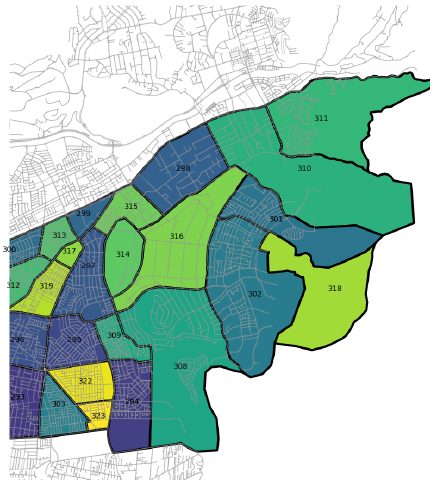
\includegraphics[width=0.5\textwidth]{fotos/mapa.png}
    \caption{Mapa de San Carlos de Apoquindo.}
    \label{fig:mapa}
\end{figure}

Para esta tarea, se generarán 3 matrices origen-destino en base a esta zonificación mediante un código Python: una utilizando el método Furness o biproporcional, con datos de los vectores origen-destino de 2024, otra a partir de una matriz de costos, como la distancia promedio de viaje, y el modelo gravitacional. Posteriormente, se calibrará la matriz con el modelo gravitacional y se compararán los resultados obtenidos con un error cuadrático medio respecto a la matriz original. Finalmente, a la matriz calibrada se le aplicará el método de Furness para obtener una matriz de viajes.

\newpage

\section{Resultados y Discusiones}
Los cálculos se realizaron en Python, utilizando las librerías Pandas y Numpy. El código se encuentra en el repositorio de GitHub \href{https://github.com/berckanala/T3_autitos/blob/main/t3.py}{Código}
\subsection{Matriz Origen-Destino con el Método Furness}
Para poder generar la Matriz Origen-Destino con el método Furness, se utilizó de base la Matriz Origen-Destino de 2012 (Tabla \ref{table:data_matrix}) y los vectores de origen y destino de 2024 (Tabla \ref{table:oi_dj_2024}). 


    
Luego, mediante el método Furness o biproporcional, que se muestra a continuación:

\begin{lstlisting}[language=Python, label= {lst:furness}]
    def furness(t, O, D, tol=1e-6, maxit=1000):  
    k = len(O)
    O = np.array(O)[:, np.newaxis].astype(float)
    D = np.array(D).astype(float)
    t = np.array(t)
    ai = np.ones((k, 1))
    bj = np.ones((1, k))
    iters = 0
    while iters < maxit:
        row_sums = t.sum(axis=1)
        col_sums = t.sum(axis=0)
        row_sums[row_sums == 0] = 1
        col_sums[col_sums == 0] = 1
        ai = O / row_sums[:, np.newaxis]
        t = t * ai
        col_sums = t.sum(axis=0)
        col_sums[col_sums == 0] = 1
        bj = D / col_sums
        t = t * bj
        row_sums_after = t.sum(axis=1)
        col_sums_after = t.sum(axis=0)
        
        if np.max(np.abs(row_sums_after - O.squeeze())) < tol and \
           np.max(np.abs(col_sums_after - D)) < tol:
            print(f"Convergencia alcanzada en {iters + 1} iteraciones.")
            break
        iters += 1
    return t
\end{lstlisting}

En donde, $t$ es la matriz origen-destino de 2012, $O$ es el vector origen de 2024 y $D$ es el vector destino de 2024. Se obtuvo la matriz origen-destino de 2024, la cual se muestra en la Tabla \ref{table:oi_dj_2024_rounded_2dp}.

\newpage

\begin{table}[h!]
    \centering
    \resizebox{\textwidth}{!}{%
    \begin{tabular}{c|ccccccccccc}
    \textbf{Zona O\textbackslash D} & \textbf{301} & \textbf{302} & \textbf{308} & \textbf{314} & \textbf{316} & \textbf{318} & \textbf{E1} & \textbf{E2} & \textbf{E3} & \textbf{E4} & \textbf{Oi,2024} \\ \hline
    \textbf{301} & 0.00 & 345.54 & 0.00 & 0.00 & 0.00 & 0.00 & 1503.36 & 0.00 & 1685.14 & 4666.00 & 8200.04 \\ 
    \textbf{302} & 0.00 & 527.75 & 0.00 & 0.00 & 389.22 & 0.00 & 1543.41 & 0.00 & 7356.23 & 6175.42 & 15992.03 \\
    \textbf{308} & 0.00 & 0.00 & 66.62 & 0.00 & 0.00 & 0.00 & 0.00 & 0.00 & 3228.47 & 3733.81 & 7028.91 \\ 
    \textbf{314} & 0.00 & 0.00 & 0.00 & 0.00 & 0.00 & 0.00 & 0.00 & 2337.00 & 0.00 & 0.00 & 2337.00 \\ 
    \textbf{316} & 0.00 & 589.60 & 0.00 & 0.00 & 0.00 & 0.07 & 144.23 & 0.00 & 2970.15 & 985.77 & 4689.82 \\ 
    \textbf{318} & 0.00 & 0.00 & 0.00 & 0.00 & 0.00 & 0.00 & 0.00 & 0.00 & 0.00 & 0.00 & 0.00 \\ 
    \textbf{E1} & 1244.34 & 787.18 & 287.07 & 4.91 & 287.66 & 0.30 & 0.00 & 0.00 & 0.00 & 0.00 & 2611.46 \\ 
    \textbf{E2} & 0.00 & 682.56 & 0.00 & 0.35 & 269.90 & 0.00 & 0.00 & 0.00 & 0.00 & 0.00 & 952.80 \\
    \textbf{E3} & 160.43 & 959.73 & 1373.06 & 6.03 & 724.61 & 0.19 & 0.00 & 0.00 & 0.00 & 0.00 & 3224.05 \\ 
    \textbf{E4} & 339.22 & 1843.65 & 3268.25 & 8.71 & 629.62 & 0.43 & 0.00 & 0.00 & 0.00 & 0.00 & 6089.88 \\ 
    \textbf{Dj, 2024} & 1744.00 & 5736.00 & 4995.00 & 20.00 & 2301.00 & 1.00 & 3191.00 & 2337.00 & 15240.00 & 15561.00 & 51126.00 \\ 
    \end{tabular}%
    }
    \caption{Matriz Origen-Destino de 2024 con el método Furness.}
    \label{table:oi_dj_2024_rounded_2dp}
\end{table}
    
Como se puede apreciar, la matriz obtenida no se igualó en columna Oi,2024 del vector de origen de 2024, pero sí el de Dj,2024. Esto se debe a que la fila de 318 no tiene viajes de origen, por lo que es imposible que se pueda llegar a la cantidad establecida en el vector de la tabla \ref{table:oi_dj_2024}. Esto repercute en el resto de la matriz, ya que al iterar, la fila de 318 no se modifica, lo que afecta a las demás filas.

\subsection{Matriz Origen-Destino con el Modelo Gravitacional}
Para poder generar la Matriz Origen-Destino con el modelo gravitacional, se utilizó la matriz de costos entre zonas (Tabla \ref{table:costs_zones}) y los vectores de origen y destino de 2012 (Tabla \ref{table:oi_dj_2012}). Luego, con la siguiente ecuación: 

\begin{equation}
    T_{ij} = \alpha \cdot O_{i,2012} \cdot D_{j,2012} \cdot C_{ij}^k \cdot e^{-\beta \cdot C_{ij}}
\end{equation}

Donde:
\begin{itemize}
    \item $T_{ij}$ es la cantidad de viajes entre la zona i y la zona j.
    \item $O_{i,2012}$ es la cantidad de viajes de origen en la zona i.
    \item $D_{j,2012}$ es la cantidad de viajes de destino en la zona j.
    \item $C_{ij}$ es el costo entre la zona i y la zona j.
    \item $\alpha$ y k son parámetros a calibrar.
    \item $\beta$ es un parámetro equivalente a 0.2176
\end{itemize}


Luego de calcular la matriz de viajes, con un $\alpha$ igual a 0.0002 y un k igual a 1
\newpage
\begin{table}[h!]
    \centering
    \resizebox{\textwidth}{!}{%
    \begin{tabular}{c|ccccccccccc}
    \textbf{Zona O\textbackslash D} & \textbf{301} & \textbf{302} & \textbf{308} & \textbf{314} & \textbf{316} & \textbf{318} & \textbf{E1} & \textbf{E2} & \textbf{E3} & \textbf{E4} & \textbf{Oi,2024} \\ \hline
    \textbf{301} & 394.66 & 5226.93 & 1499.56 & 1429.52 & 739.23 & 356.11 & 1208.32 & 631.28 & 1639.95 & 1179.97 & 14305.53 \\ 
    \textbf{302} & 3424.46 & 13095.60 & 6443.93 & 3896.18 & 1886.55 & 1703.88 & 4011.18 & 1909.91 & 5919.04 & 4478.56 & 46769.28 \\ 
    \textbf{308} & 2536.04 & 16633.99 & 3421.34 & 2900.77 & 1731.41 & 2007.81 & 3427.09 & 1535.92 & 5417.51 & 4475.28 & 44087.17 \\ 
    \textbf{314} & 17.74 & 73.82 & 21.29 & 6.51 & 6.56 & 10.83 & 19.98 & 7.95 & 25.11 & 23.13 & 212.91 \\ 
    \textbf{316} & 1457.93 & 5679.12 & 2019.14 & 1041.82 & 521.16 & 897.38 & 1788.74 & 763.11 & 2268.53 & 1921.72 & 18358.65 \\ 
    \textbf{318} & 0.29 & 2.14 & 0.97 & 0.72 & 0.37 & 0.13 & 0.61 & 0.31 & 0.82 & 0.62 & 6.98 \\ 
    \textbf{E1} & 731.01 & 3703.98 & 1225.96 & 973.71 & 548.70 & 450.59 & NaN & NaN & NaN & NaN & 7633.95 \\ 
    \textbf{E2} & 766.05 & 3537.55 & 1102.08 & 777.63 & 469.53 & 461.63 & NaN & NaN & NaN & NaN & 7114.48 \\ 
    \textbf{E3} & 4720.63 & 26006.23 & 9221.03 & 5822.74 & 3310.98 & 2884.16 & NaN & NaN & NaN & NaN & 51965.78 \\ 
    \textbf{E4} & 1836.03 & 10636.64 & 4117.56 & 2899.79 & 1516.16 & 1174.92 & NaN & NaN & NaN & NaN & 22181.10 \\ 
    \textbf{Dj, 2024} & 15884.85 & 84596.00 & 29072.87 & 19749.39 & 10730.65 & 9947.44 & 10455.92 & 4848.49 & 15270.95 & 12079.28 & 212635.84 \\ 
    \end{tabular}
    }
    \caption{Matriz de viajes obtenida con el modelo gravitacional.}
    \label{table:matrix_nan_sums_corrected}
\end{table}
    
Luego, se obtuvo una matriz la cual se le calculó el error cuadrático medio respecto a la original con el siguiente código:


\begin{lstlisting}
    mse = np.mean((Tij_df - df1_1) ** 2)
\end{lstlisting}

En donde, $Tij\_df$ es la matriz de viajes obtenida y $df1\_1$ es la matriz original. Se obtuvo un error cuadrático medio de 13711172.376, lo que indica que la matriz obtenida no es precisa respecto a la original. Por esta razón se fue modificando el valor de k para minimizar el error, se ocupó un k de 0.001 obteniendo un error de 1968630.51. 

\subsection{Calibración de la Matriz Origen-Destino con el Modelo Gravitacional}

Para poder obtener esta matriz, lo que se hizo fue con la matriz obtenido anteriormente (Tabla \ref{table:matrix_nan_sums_corrected}), se le aplicó el método Furness (\ref{lst:furness}), obteniendo una matriz de viajes calibrada. Esta matriz en comparación con las anteriores, se obtuvo un error de 0 en los vectores de la matriz.

\begin{table}[h!]
    \centering
    \resizebox{\textwidth}{!}{%
    \begin{tabular}{c|ccccccccccc}
    
    \textbf{Zona O\textbackslash D} & \textbf{301} & \textbf{302} & \textbf{308} & \textbf{314} & \textbf{316} & \textbf{318} & \textbf{E1} & \textbf{E2} & \textbf{E3} & \textbf{E4} & \textbf{Oi,2024} \\ \hline
    \textbf{301} & 121.45 & 257.94 & 205.80 & 0.53 & 83.77 & 0.07 & 676.48 & 658.35 & 2830.91 & 2901.71 & 7737.00 \\ 
    \textbf{302} & 142.46 & 455.73 & 251.41 & 1.02 & 151.92 & 0.09 & 1180.06 & 836.05 & 6111.30 & 5958.95 & 15089.00 \\ 
    \textbf{308} & 53.60 & 118.55 & 120.62 & 0.39 & 50.51 & 0.03 & 433.54 & 256.99 & 2870.58 & 2727.19 & 6632.00 \\ 
    \textbf{314} & 12.96 & 44.74 & 36.40 & 0.17 & 19.43 & 0.01 & 227.24 & 113.43 & 830.97 & 1022.65 & 2308.00 \\ 
    \textbf{316} & 34.71 & 113.98 & 80.36 & 0.33 & 45.39 & 0.02 & 430.84 & 271.41 & 1599.70 & 1848.25 & 4425.00 \\ 
    \textbf{318} & 41.76 & 105.47 & 63.33 & 0.20 & 30.80 & 0.03 & 242.84 & 200.77 & 996.54 & 1102.26 & 2784.00 \\ 
    \textbf{E1} & 301.57 & 952.48 & 742.11 & 4.18 & 463.48 & 0.17 & 0.00 & 0.00 & 0.00 & 0.00 & 2464.00 \\ 
    \textbf{E2} & 154.99 & 356.35 & 232.30 & 1.10 & 154.18 & 0.07 & 0.00 & 0.00 & 0.00 & 0.00 & 899.00 \\ 
    \textbf{E3} & 298.87 & 1168.15 & 1163.66 & 3.62 & 407.54 & 0.17 & 0.00 & 0.00 & 0.00 & 0.00 & 3042.00 \\ 
    \textbf{E4} & 581.63 & 2162.59 & 2098.99 & 8.45 & 893.99 & 0.35 & 0.00 & 0.00 & 0.00 & 0.00 & 5746.00 \\ 
    \textbf{Dj, 2024} & 1744.00 & 5736.00 & 4995.00 & 20.00 & 2301.00 & 1.00 & 3191.00 & 2337.00 & 15240.00 & 15561.00 & 51126.00 \\ 
    \end{tabular}
    }
    \caption{Matriz de viajes calibrada con el método Furness.}
    \label{table:rounded_data}
\end{table}
    



\newpage
\section{Anexos}
\begin{table}[h!]
    \centering
    \begin{tabular}{c|cccccccccc}
    
    \textbf{Zona O\textbackslash D} & \textbf{301} & \textbf{302} & \textbf{308} & \textbf{314} & \textbf{316} & \textbf{318} & \textbf{E1} & \textbf{E2} & \textbf{E3} & \textbf{E4} \\ \hline
    \textbf{301} & 0 & 0 & 0 & 0 & 0 & 0 & 709 & 0 & 714 & 821 \\ 
    \textbf{302} & 284 & 845 & 0 & 0 & 1202 & 0 & 369 & 894 & 3514 & 3671 \\ 
    \textbf{308} & 0 & 0 & 107 & 0 & 0 & 0 & 39 & 0 & 1457 & 1886 \\ 
    \textbf{314} & 0 & 0 & 0 & 0 & 0 & 0 & 126 & 25 & 1208 & 949 \\ 
    \textbf{316} & 0 & 171 & 0 & 0 & 0 & 0 & 37 & 97 & 728 & 344 \\ 
    \textbf{318} & 0 & 0 & 0 & 0 & 108 & 0 & 107 & 0 & 529 & 650 \\ 
    \textbf{E1} & 811 & 1622 & 0 & 0 & 193 & 0 & 0 & 0 & 0 & 0 \\ 
    \textbf{E2} & 98 & 836 & 0 & 25 & 0 & 0 & 0 & 0 & 0 & 0 \\ 
    \textbf{E3} & 121 & 1029 & 1563 & 0 & 529 & 0 & 0 & 0 & 0 & 0 \\ 
    \textbf{E4} & 645 & 1663 & 3480 & 0 & 338 & 0 & 0 & 0 & 0 & 0 \\ 
    \end{tabular}
    \caption{Matriz Origen-Destino de 2012}
    \label{table:data_matrix}
\end{table}

\begin{table}[h!]
    \centering
    \begin{tabular}{c|ccccccccccc}
    
    \textbf{Zona} & \textbf{301} & \textbf{302} & \textbf{308} & \textbf{314} & \textbf{316} & \textbf{318} & \textbf{E1} & \textbf{E2} & \textbf{E3} & \textbf{E4} \\ \hline
    \textbf{Oi,2012} & 1960 & 6166 & 5150 & 25 & 2371 & 1 & 1387 & 1016 & 8150 & 8322 \\ 
    \textbf{Dj,2012} & 2245 & 10780 & 3488 & 2307 & 1377 & 1395 & 2626 & 959 & 3243 & 6126 \\
    \end{tabular}
    \caption{Vectores de Oi,2012 y Dj,2012 por zona}
    \label{table:oi_dj_2012}
    \end{table}
    
    
\begin{table}[h!]
    \centering
    \begin{tabular}{c|cccccccccc}
    
    \textbf{Zona} & \textbf{301} & \textbf{302} & \textbf{308} & \textbf{314} & \textbf{316} & \textbf{318} & \textbf{E1} & \textbf{E2} & \textbf{E3} & \textbf{E4} \\ \hline
    \textbf{Oi,2024} & 7737 & 15089 & 6632 & 2308 & 4425 & 2784 & 2464 & 899 & 3042 & 5746 \\ 
    \textbf{Dj,2024} & 1744 & 5736 & 4995 & 20 & 2301 & 1 & 3191 & 2337 & 15240 & 15561 \\ 
    \end{tabular}
    \caption{Vectores $O_{i2024}$ y $D_{j2024}$ por zona}
    \label{table:oi_dj_2024}
\end{table}


\begin{table}[h!]
    \centering
    \begin{tabular}{c|cccccccccc}
    
    \textbf{Zona O\textbackslash D} & \textbf{301} & \textbf{302} & \textbf{308} & \textbf{314} & \textbf{316} & \textbf{318} & \textbf{E1} & \textbf{E2} & \textbf{E3} & \textbf{E4} \\ \hline
    \textbf{301} & 0.50 & 1.85 & 1.53 & 3.11 & 2.22 & 0.77 & 9.71 & 5.15 & 8.85 & 16.01 \\ 
    \textbf{302} & 1.85 & 1.31 & 2.69 & 2.22 & 1.56 & 1.32 & 9.23 & 6.13 & 7.39 & 14.78 \\ 
    \textbf{308} & 1.53 & 2.69 & 1.25 & 1.81 & 1.81 & 2.31 & 9.02 & 6.74 & 6.05 & 13.56 \\ 
    \textbf{314} & 3.11 & 2.22 & 1.81 & 0.65 & 1.25 & 2.95 & 7.04 & 5.55 & 6.80 & 13.12 \\ 
    \textbf{316} & 2.22 & 1.56 & 1.81 & 1.25 & 0.99 & 2.18 & 7.74 & 5.18 & 7.43 & 14.04 \\ 
    \textbf{318} & 0.77 & 1.32 & 2.31 & 2.95 & 2.18 & 0.50 & 9.78 & 5.97 & 9.01 & 15.82 \\ 
    \textbf{E1} & 9.71 & 9.23 & 9.02 & 7.04 & 7.74 & 9.78 & $\infty$ & $\infty$ & $\infty$ & $\infty$ \\ 
    \textbf{E2} & 5.15 & 6.13 & 6.74 & 5.55 & 5.18 & 5.97 & $\infty$ & $\infty$ & $\infty$ & $\infty$ \\ 
    \textbf{E3} & 8.85 & 7.39 & 6.05 & 6.80 & 7.43 & 9.01 & $\infty$ & $\infty$ & $\infty$ & $\infty$ \\ 
    \textbf{E4} & 16.01 & 14.78 & 13.56 & 13.12 & 14.04 & 15.82 & $\infty$ & $\infty$ & $\infty$ & $\infty$ \\ 
    \end{tabular}
    \caption{Tabla de costos entre zonas}
    \label{table:costs_zones}
\end{table}
    


\end{document}
